\appendix
%
% If you only have one appendix, you should change the above to:
%\appendix
%

\chapter{}

\begin{figure}[H]
    \centering
    \begin{tabular}{lcc}
        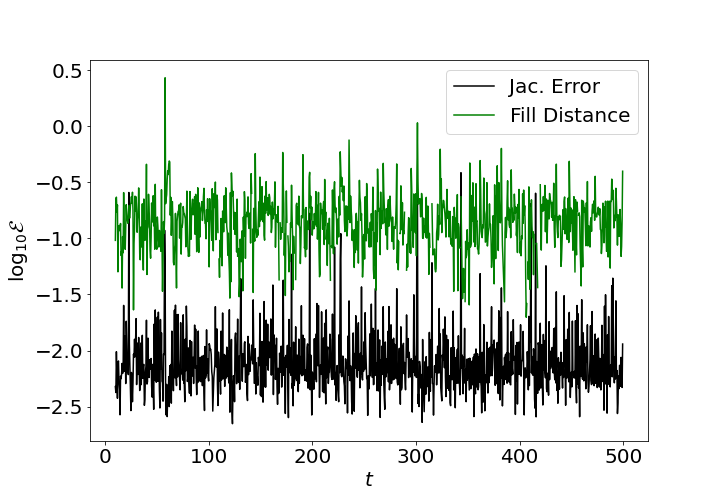
\includegraphics[width=6.5cm]{/Jacobian Error/Lorenz, t=500.png}&
        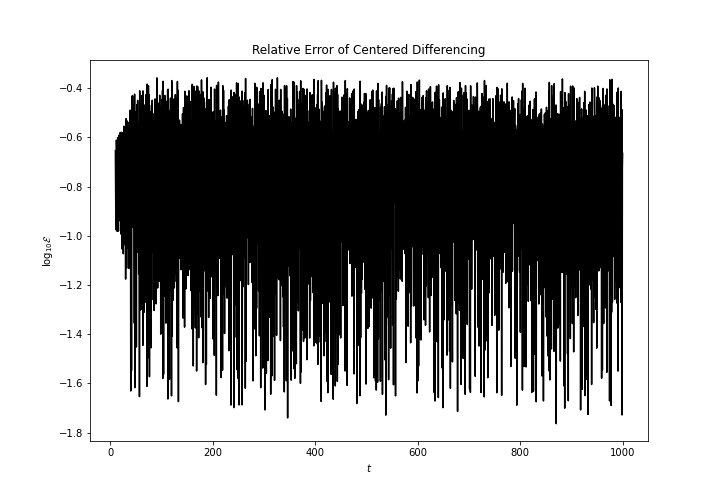
\includegraphics[width=6.5cm]{/Jacobian Error/Lorenz, dt=0,1.png}\\
        \hfil a &b\\
        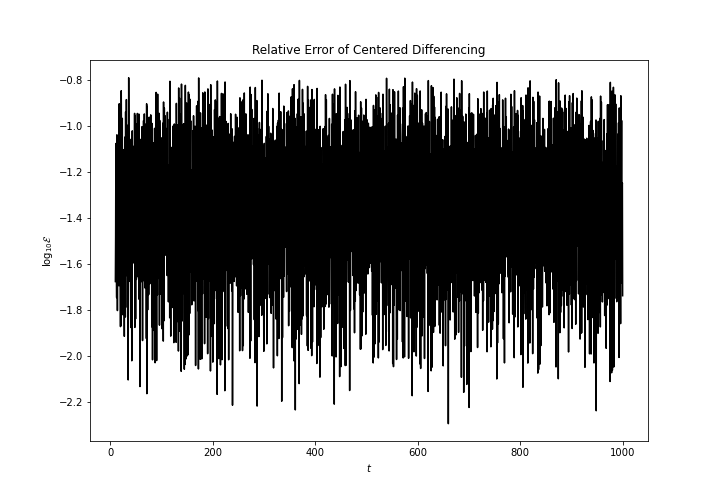
\includegraphics[width=6.5cm]{/Jacobian Error/Lorenz, dt=0,05.png}&
        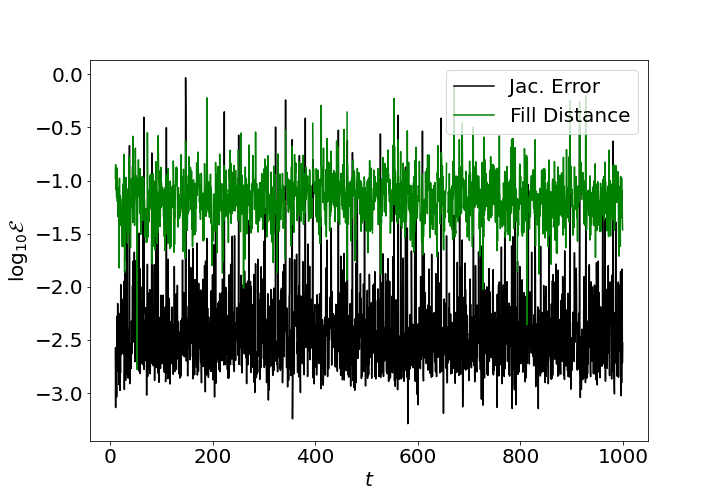
\includegraphics[width=6.5cm]{/Jacobian Error/Lorenz, dt=0,005.png}\\
        \hfil c &d\\
    \end{tabular}
    \caption{Lorenz Jacobian Error and Fill Distance, a. $t=500$, $dt=0.01$ b. $t=1000$, $dt=0.1$ c. $t=1000$, $dt=0.05$ d. $t=1000$, $dt=0.005$}\label{fig:lorenzjac2}
\end{figure}

\begin{figure}[H]
    \centering
    \begin{tabular}{lcc}
        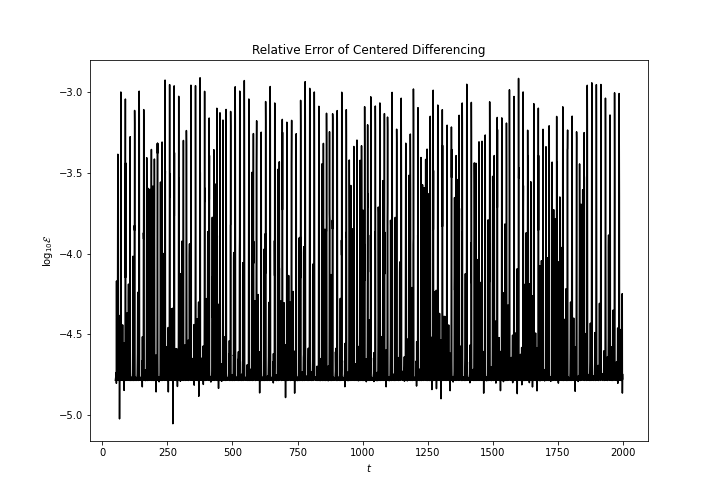
\includegraphics[width=6.5cm]{/Jacobian Error/Rossler, t=2000.png}&
        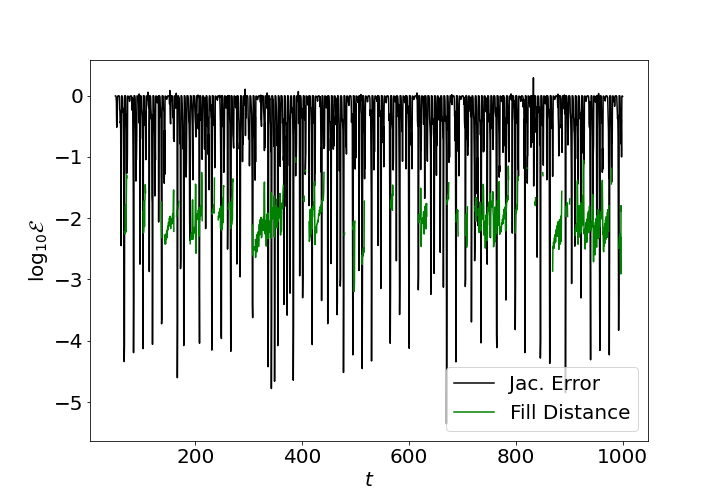
\includegraphics[width=6.5cm]{/Jacobian Error/Rossler, dt=0,1.png}\\
        \hfil a &b\\
        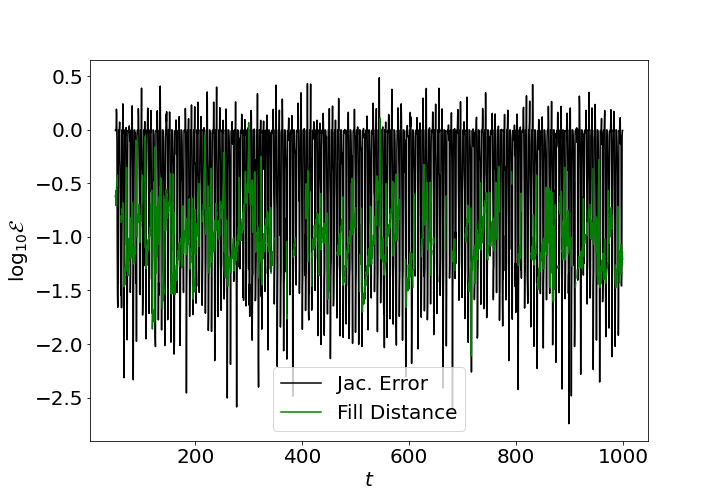
\includegraphics[width=6.5cm]{/Jacobian Error/Rossler, dt=0,05.png}&
        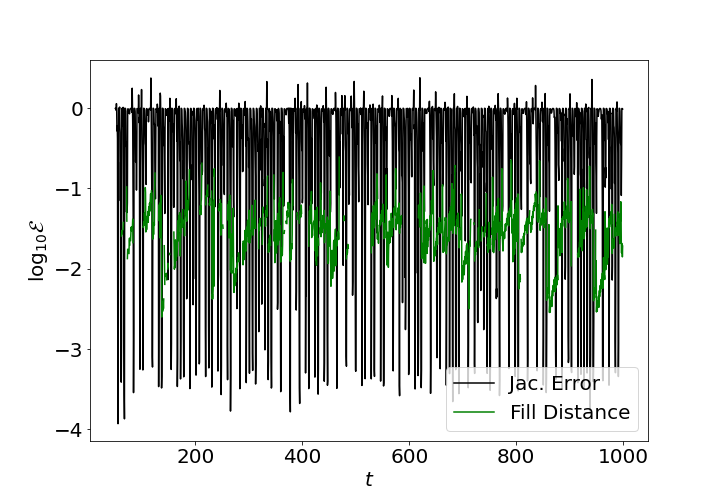
\includegraphics[width=6.5cm]{/Jacobian Error/Rossler, dt=0,005.png}\\
        \hfil c &d\\
    \end{tabular}
    \caption{Rossler Jacobian Error and Fill Distance, a. $t=2000$, $dt=0.01$ b. $t=1000$, $dt=0.1$ c. $t=1000$, $dt=0.05$ d. $t=1000$, $dt=0.005$}\label{fig:rosslerjac2}
\end{figure}

